\section{Introduction}
\label{sec:introduction}

Historical questions often ask about a period, while sources give only approximate event dates.
A source might report an appointment in September without identifying its day.
Choosing the first or last day can change which evidence reaches a reader.
Yet resolving every uncertain date wastes effort when those dates cannot change the selected context.
We ask a practical question:
\emph{When does date uncertainty actually change retrieval?}

This problem arises before answer generation.
Retrieval-augmented systems must select a few excerpts from longer histories~\citep{lewis2020rag}.
Consider the presenters of a television programme during a transition month.
The source names both presenters and dates their succession only to that month.
The previous presenter may contribute evidence for part of the requested period.
A single guessed transition date conceals that uncertainty.
A question covering the entire transition month can instead have a stable evidence set.
The distinction depends on the question's scope and the context budget.

\begin{figure*}[t]
\centering
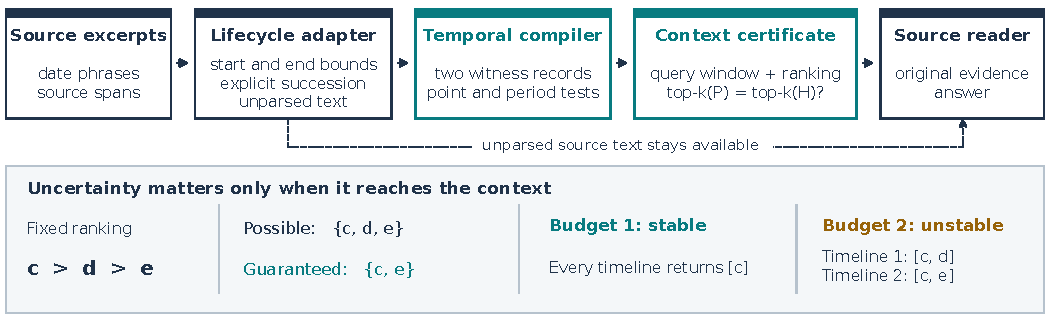
\includegraphics[width=\textwidth]{figures/architecture.pdf}
\caption{Source spans become dated claims with explicit replacement decisions. Two witnesses per claim support exact temporal tests. A fixed ranking then yields a stable context or two admissible timelines with different contexts. Unparsed source text follows a shared fallback policy.}
\label{fig:architecture}
\end{figure*}

Temporal memories already preserve histories and invalidate replaced facts.
Graphiti applies direct contradiction decisions~\citep{rasmussen2025zep,graphiti2026source}.
NuggetIndex maintains atomic evidence, validity intervals, and lifecycle states~\citep{zerhoudi2026nuggetindex}.
DeFuzzRAG and IA-RAG address fuzzy dates and interval retrieval~\citep{chen2026defuzzrag,wang2026iarag}.
We study the decisions available before completing uncertain dates.
The goal is an exact, inspectable interface between temporal evidence and ranked retrieval.

Each claim receives a range containing its unknown start date.
A directed decision specifies which other claims can replace it.
We compile these inputs into at most two source witnesses per claim.
The first determines when support becomes impossible.
The second determines when guaranteed support can fail.
They answer every point or period query without enumerating timelines.
\emph{Possible support} means that a claim applies somewhere in the requested period under at least one allowed timeline.
\emph{Guaranteed support} means that it applies somewhere in that period under every allowed timeline.

The resulting masks also decide whether uncertainty changes retrieval.
Fix a relevance ranking and a budget of $k$ claims.
If its first $k$ possible claims are guaranteed, every timeline returns the same context.
Otherwise, we identify a selected claim whose membership changes across two explicit timelines.
These timelines can be replayed through the retrieval pipeline.
They identify which dates need clarification.

Our contributions are threefold.
First, we derive exact period-support formulas and a sharp two-witness representation.
Compilation takes linear time in the claims and supplied replacement pairs.
Second, we characterize context stability and construct witnesses when it fails.
Date refinement preserves settled decisions, while each changed replacement pair affects only its target.
We also separate tractable stability certification from NP-hard possible context membership.
Third, we implement source-span extraction, explicit endpoints, matched date completions, and a local reader.
Natural-source experiments measure extraction coverage, context ambiguity, and answer behavior under shared inputs.
Complete-answer snapshot controls establish the costs of discarding alternatives before selection.
